\documentclass[aspectratio=169, 10pt]{beamer} % dvipsnames gives more built-in colors
\usepackage{preamble}
\usepackage{hyperref}
\usepackage{array}
\usepackage{mathtools}
\usepackage{amsmath, array}
\DeclareMathOperator*{\argmax}{arg\,max}
%\usepackage{epsfig}
\usepackage{makecell,multirow,diagbox} 
\usepackage{verbatim}
\usepackage{enumerate}
\usepackage{booktabs}
\usepackage{tabularx}
\usepackage{graphicx}
\usepackage{slashbox,multirow}
\usepackage{epstopdf}
\usepackage{placeins}
\usepackage{algorithmicx}
\usepackage{amssymb}
\usepackage{mathtools}
\usepackage{color, colortbl}
\usepackage{siunitx}
\usepackage{threeparttable}
\usepackage{bm}
\usepackage[compatibility=false, font=footnotesize]{caption}
\usepackage{subcaption}
\usepackage{amssymb}
\usepackage{pifont}
\usepackage{eurosym}

% ready for the next
\title{Offshore Wind Park Optimization}
\institute{\large{\textbf{Escola Tècnica Superior d'Enginyeria Industrial de Barcelona (ETSEIB)}} \\[1.5ex]
\large{\textbf{Universitat Pompeu Fabra (UPF)}} \\[1.5ex]
{Bachelor's Degree in Industrial Technologies and Economic Analysis}}
\date{July 2024}
\author[Carles Roca]{Carles Roca Reverter}
\subject{Bachelor's Degree in Industrial Technologies and Economic Analysis}



% ---content---
\begin{document}

\begin{frame}[plain]
\hspace*{-1.0cm}\parbox[t]{\textwidth}{
	\titlepage
    } 
\end{frame}

\begin{frame}{Contents}
	\footnotesize
	\tableofcontents
\end{frame}



\section{Introduction}

\begin{frame}{}
    \tableofcontents[currentsection]
\end{frame}


% \subsection{Motivation}
\begin{frame}{Motivation}
\begin{itemize}
    \item Variable renewable energy like wind and solar is becoming increasingly prevalent in the electrical grid.
    \item The presence of these sources is leads to unwanted effects in the grid such as overvoltages and voltage imbalances.  
    \item Historic solutions are not well equipped to deal with these effects and especially the fast response times required.
    \item New power electronics based solutions, such as the unified power quality converter (UPQC), are investigated to solve this problem.
\end{itemize}
\end{frame}


% \subsection{Goals}
\begin{frame}{Goals}
\begin{itemize}
\item To analyze voltage spread of distribution grid with high penetration of solar.
\item To develop a dynamic model of the UPQC, including all required controllers.
\item To develop an equivalent static model of the UPQC and validate its behaviour with the dynamic model.
\item To propose design methodology for the converter sizing making use of the developed tools.
\item To show behaviour of the converter over sample days using different design criteria.
\end{itemize}
\end{frame}


\section{Transmission system model}


\begin{frame}{}
    \tableofcontents[currentsection]
\end{frame}



\begin{frame}{Transmission system design}
  Converters are prone to be saturated during short-circuits ($I_{max}$ is reached). 

\begin{table}[!htb]\centering
  \caption{Possible operating states of the converters in grid-following mode.}
  \begin{tabular}{ccc}
    \hline
    \textbf{Converter State} & \textbf{PQ} & \textbf{PV} \\
    \hline
    \hline
    USS & $P$, $Q$ & $P$, $V$ \\
    PSS & $Q$, $I_{max}$ & $V$, $I_{max}$ \\
    FSS & $P=0$, $I_{max}$ & $P=0$, $I_{max}$ \\
    DIS & $P=0$, $Q=0$ & $P=0$, $Q=0$ \\
    \hline
  \end{tabular}
  \label{tab:convs1}
\end{table}

\end{frame}

\subsection{Elements modelling}


\begin{frame}{Elements modelling}
Traditional power flow:
\begin{equation}
  \begin{pmatrix}
    \bm{\Delta f}_P \\
    \bm{\Delta f}_Q \\
  \end{pmatrix} = -
  \begin{pmatrix}
    \frac{d \bm{f}_P}{d \bm{\theta}} & \frac{d \bm{f}_P}{d \bm{\nu}} \\
    \frac{d \bm{f}_Q}{d \bm{\theta}} & \frac{d \bm{f}_Q}{d \bm{\nu}} \\
  \end{pmatrix}
  \begin{pmatrix}
    \bm{\Delta \theta} \\
    \bm{\Delta \nu} \\
  \end{pmatrix}.
  \label{eq:syst2xx}
\end{equation}

Extended Newton-Raphson considering current saturation:
\begin{equation}
  \begin{pmatrix}
    \bm{\Delta f_P} \\
    \bm{\Delta f_Q} \\
    \bm{\Delta f_{I^2}} \\
  \end{pmatrix} = -
  \begin{pmatrix}
    \frac{d \bm{f_P}}{d \bm{\theta}} & \frac{d \bm{f_P}}{d \bm{\nu}} \\
    \frac{d \bm{f_Q}}{d \bm{\theta}} & \frac{d \bm{f_Q}}{d \bm{\nu}} \\
    \frac{d \bm{f_{I^2}}}{d \bm{\theta}} & \frac{d \bm{f_{I^2}}}{d \bm{\nu}} \\
  \end{pmatrix}
  \begin{pmatrix}
    \bm{\Delta \theta} \\
    \bm{\Delta \nu} \\
  \end{pmatrix},
  \label{eq:systfin}
\end{equation}
where the residuals are:
\begin{equation}
  \begin{cases}
    \bm{\Delta f_P} = -\bm{P}_\text{set} + \Re([\bm{V}]\bm{Y}^*\bm{V}^*),\\
    \bm{\Delta f_Q} = -\bm{Q}_\text{set} + \Im([\bm{V}]\bm{Y}^*\bm{V}^*),\\
  \bm{\Delta f}_{I^2} =  \bm{I_c} \bm{I_c}^* = - \bm{I}_{c,max}^2 + (\bm{Y}\bm{V} - [\bm{V}^*]^{-1} \bm{S}^* - \bm{I_l}) \cdot (\bm{Y}\bm{V} - [\bm{V}^*]^{-1} \bm{S}^* - \bm{I}_l)^*.
\end{cases}
\end{equation}
\end{frame}

\begin{frame}{New bus types}
New categories of buses emerge:

\begin{table}[!htb]\centering
  \caption{Traditional types of buses and mapping to new buses depending on the converter state.}
  \begin{tabular}{ccc}
    \hline
    \textbf{Converter State} & \textbf{PQ Control} & \textbf{PV Control} \\
    \hline
    \hline
    USS & PQ & PV \\
    PSS & QI & VI \\
    FSS & PI & PI \\
    DIS & PQ & PQ \\
    \hline
  \end{tabular}
  \label{tab:stat}
\end{table}

\end{frame}



\subsection{Cost modelling}

\begin{frame}{Costs}

\begin{figure}[!htb]\centering
\incfig{texas3}
\caption{Approximate location of the three converters.}
\label{fig:texas}
\end{figure}

\end{frame}


\begin{frame}{Summary}
\begin{table}[!htb]\centering \footnotesize
  \caption{Power flow results for the converters under normal conditions.}
  \begin{tabular}{cccccccc}
    \hline
    \textbf{VSC} & \textbf{State} & $\bm{\nu}$ & $\bm{\theta}$ ($^{\circ}$) & $|\bm{I}|$ & $\bm{P}$ & $\bm{Q}$ & $|\bm{S}|$ \\
    \hline
    \hline
    vsc1 & \cellcolor{gray!40}USS & 1.0073 & -40.7924 & \cellcolor{gray!40}5.8017 & -5.0000 & 3.0260 & 5.8443 \\
    vsc2 & \cellcolor{gray!40}USS & 1.0050 & -63.9565 & \cellcolor{gray!40}1.3882 & -1.0000 & 0.9731 & 1.3953 \\
    vsc3 & \cellcolor{gray!40}USS & 1.0200 & -48.6301 & \cellcolor{gray!40}6.0529 & 6.0000 & 1.4580 & 6.1746 \\
    \hline
  \end{tabular}
  \label{tab:2000_1}
\end{table}

\begin{table}[!htb]\centering \footnotesize
  \caption{Short-circuit results for the converters with $\underline{Z}_f=0.002j$.}
  \begin{tabular}{cccccccc}
    \hline
    \textbf{VSC} & \textbf{State} & $\bm{\nu}$ & $\bm{\theta}$ ($^{\circ}$) & $|\bm{I}|$ & $\bm{P}$ & $\bm{Q}$ & $|\bm{S}|$ \\
    \hline
    \hline
    vsc1 & \cellcolor{gray!40}FSS & 0.0633 & -14.1576 & \cellcolor{gray!40}7.0000 & 0.0000 & 0.4431 & 0.4431 \\
    vsc2 & \cellcolor{gray!40}USS & 0.9997 & -63.3836 & \cellcolor{gray!40}1.3958 & -1.0000 & 0.9732 & 1.3954 \\
    vsc3 & \cellcolor{gray!40}USS & 0.9997 & -46.1701 & \cellcolor{gray!40}6.1764 & 6.0000 & 1.4582 & 6.1746 \\
    \hline
  \end{tabular}
  \label{tab:2000_2}
\end{table}

\begin{table}[!htb]\centering \footnotesize
  \caption{Short-circuit results for the converters with $\underline{Z}_f=0.05j$.}
  \begin{tabular}{cccccccc}
    \hline
    \textbf{VSC} & \textbf{State} & $\bm{\nu}$ & $\bm{\theta}$ ($^{\circ}$) & $|\bm{I}|$ & $\bm{P}$ & $\bm{Q}$ & $|\bm{S}|$ \\
    \hline
    \hline
    vsc1 & \cellcolor{gray!40}PSS & 0.6423 & -34.1962 & \cellcolor{gray!40}7.0000 & -3.1009 & 3.2557 & 4.4962 \\
    vsc2 & \cellcolor{gray!40}USS & 1.0050 & -63.9565 & \cellcolor{gray!40}1.3882 & -1.0000 & 0.9696 & 1.3928 \\
    vsc3 & \cellcolor{gray!40}USS & 1.0200 & -48.6301 & \cellcolor{gray!40}6.0529 & 6.0000 & 1.4453 & 6.1716 \\
    \hline
  \end{tabular}
  \label{tab:2000_3}
\end{table}
\end{frame}

\begin{frame}{Results validation}
 \begin{figure}[!htb]\centering
  \begin{subfigure}{0.45\textwidth}
    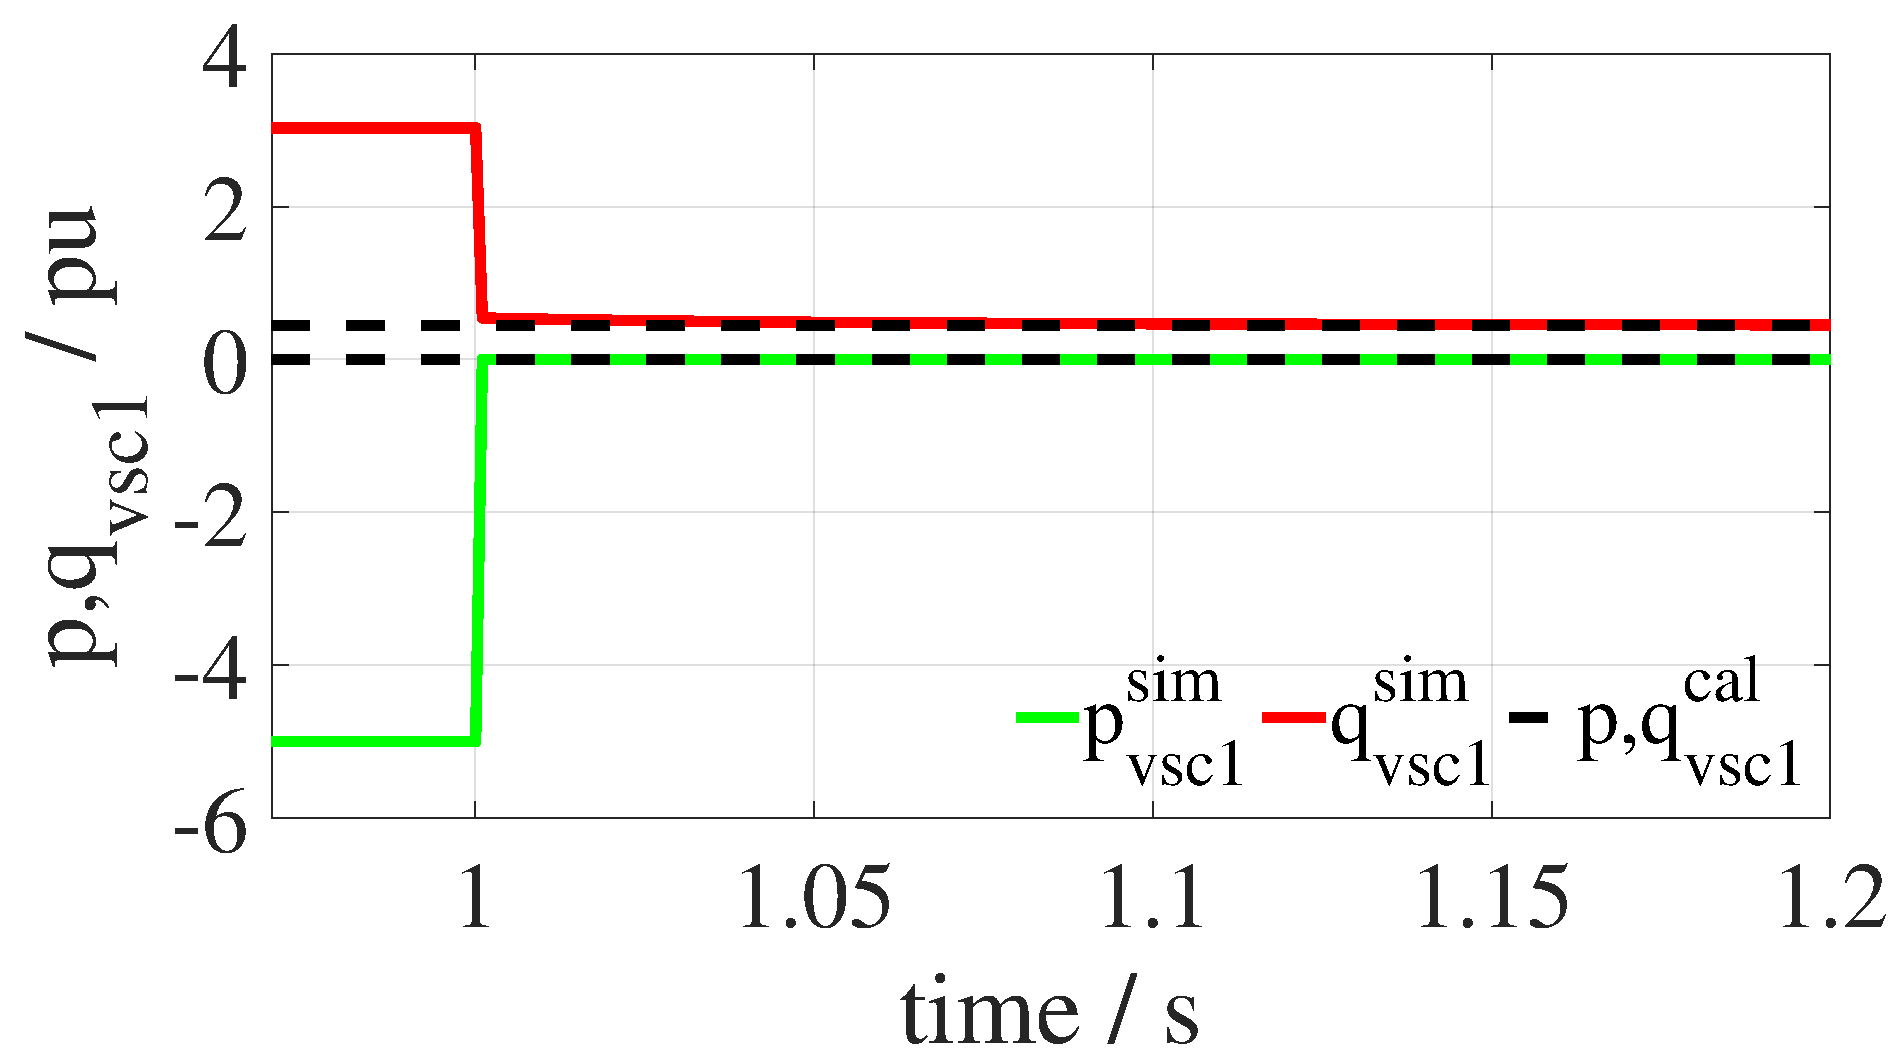
\includegraphics[width=6.0cm]{Data/psim_z0002.pdf}
    \caption{VSC1 power injections.}
  \end{subfigure}
  \begin{subfigure}{0.45\textwidth}
    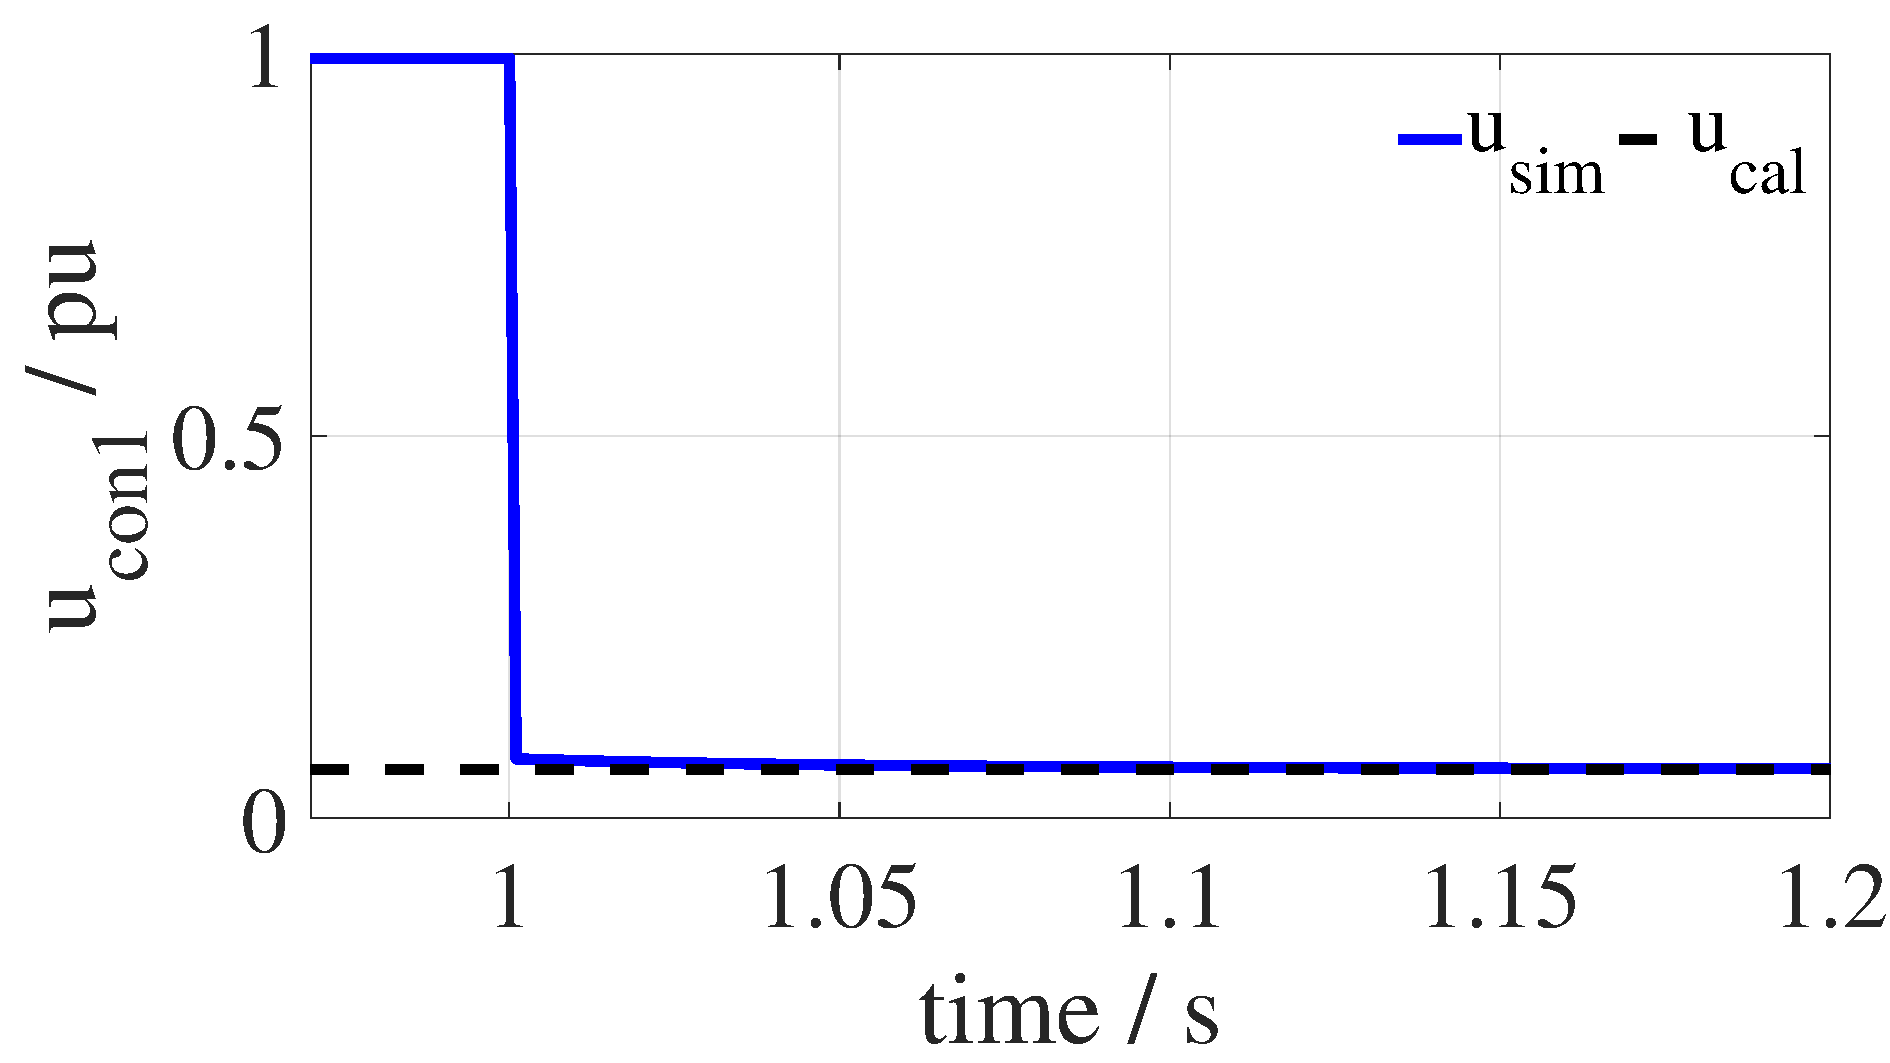
\includegraphics[width=6.0cm]{Data/usim_z0002.pdf}
    \caption{Fault voltage.}
  \end{subfigure}
	\caption{Dynamic simulation with PSS/E for a severe fault with $\underline{Z}_{f}=j0.002$ pu.}
    \label{fig:dyn1}
\end{figure}   
\end{frame}

\begin{frame}{Comparison with PSS/E}
  Steady-state calculations:
\begin{table}[!htb]\centering\footnotesize
	\caption{Steady-state short-circuit results with the proposed method and PSS/E.}
	\begin{tabular}{cccc}
        \hline
        \backslashbox{$\bm{\underline{Z}_{f}}$}{$\bm{I_{sc}}$} & \textbf{Proposed method} & \textbf{PSS/E VSCs as generators} & \textbf{PSS/E VSCs as FACTS} \\
        \hline
        \hline
        $j0.05$ & \cellcolor{green!30}12.75 & \cellcolor{red!30}13.40 & \cellcolor{red!30}12.17 \\
		$j0.002$ & \cellcolor{green!30}31.40 & \cellcolor{red!30}32.57 & \cellcolor{red!30}25.91 \\
        \hline
	\end{tabular}
	\label{tab:valid}
\end{table}
PSS/E dynamic simulation:
	\begin{table}[!htb]\centering\footnotesize
			\caption{Comparison of efficiency with PSS/E dynamic simulation.}
			% \begin{tabular}{m{3cm}<{\centering}|m{2.5cm}<{\centering}m{4cm}<{\centering}}
              \begin{tabular}{crr}
              \hline
              $\bm{t_{sim}}$ \textbf{after fault (s)}& \textbf{Calculation time (s)}& \textbf{Error} $|\bm{u_{sample}-u_{cal}}|$ \textbf{(pu)} \\
                \hline
                \hline
				0.3 & 1.43 & $42 \times 10^{-3}$ \\
				1 & 3.52 & $19.8 \times 10^{-3}$ \\
				2 & 6.81 & $6.5 \times 10^{-3}$ \\
				3 & 10.07 & $1.6 \times 10^{-3}$ \\
				4 & 13.14 & $<0.1 \times 10^{-3}$ \\
				\hline
                \rowcolor[gray]{0.8} Proposed method & 0.085 & $6.17 \times 10^{-11}$ \\
                \hline
			\end{tabular}
            \label{tab:comparex}
	\end{table}	

\end{frame}

% \subsection{Algebraic limits}
% \begin{frame}{Algebraic limits}
% \begin{itemize}
%     \item Up to this point, the states of converters are predetermined. 
%     \item Converters are initially assumed to be unsaturated. If no solution is obtained, they are saturated following some heuristics.
%     \item Finding a solution is not guaranteed, and multiple solutions can coexist.
%     \item Since each of the $n$ converters can operate in 4 different states (USS, PSS, FSS and DIS), there are $4^n$ possible combinations. Solving systems with many converters is a computational challenge.
% \end{itemize}
% For all these reasons, it may be a good idea to include the current limits of the converters in an algebraic manner. The system of equations could be solved at one go. 
% \end{frame}

% \begin{frame}{Formulation of the Lagrangian}
% \begin{figure}[!htb]\centering\footnotesize
%   \begin{circuitikz}[european]
%     \draw[line width=0.1cm] (0,0) to [short] (0,-0.8);
%     \draw (0,-0.4) to [/tikz/circuitikz/bipoles/length=25pt, R] (2,-0.4);
%     \draw (0,-0.2) to [/tikz/circuitikz/bipoles/length=25pt, R, l=${g}_{ij}$] (2,0.6);
%     \draw (0,-0.6) to [/tikz/circuitikz/bipoles/length=25pt, R] (2,-1.4);
%     \draw (-0.5,-0.6) to [short] (-0.0,-0.6);
%     % \draw (-0.2,-0.6) to [/tikz/circuitikz/bipoles/length=25pt, R, l_=$\underline{Y}_{sh,i}$] (-0.2,-2.5);
%   \draw (-0.5,-1) to [short, i=${I}_i$] (-0.5,-0.6);
%     \draw (-0.5,-2.5) to [american current source] (-0.5,-1.0);
%     \draw (-0.7,-2.5) to [short] (-0.3,-2.5);
%     % \draw (-2.2,-0.4) to [sdcac] (-1.2,-0.4);
%     % \draw (0,0) to [twoportsplit, t1={$=$}, t2={$=$}] ++(3,0);

%     \draw (0.4,-1) to [/tikz/circuitikz/bipoles/length=25pt, R, l=$g_{sh,i}$] (0.4,-2.4);
%     \draw (0.4, -2.4) to [short] (0.4,-2.5);
%     \draw (0.2,-2.5) to [short] (0.6,-2.5);
%     \draw (0.4,-1) to [short] (0,-0.6);

%     \draw (-2.2,-0.9) to [short] (-1.2,-0.9);
%     \draw (-1.2,0.1) to [short] (-2.2,0.1);
%     \draw (-2.2,-0.9) to [short] (-2.2,0.1);
%     \draw (-1.2,-0.9) to [short] (-1.2,0.1);
%     \draw (-2.2,0.1) to [short] (-1.2,-0.9);

%     \draw (-1.5, -0.1) to [short] (-1.3, -0.1);
%     \draw (-1.5, 0.0) to [short] (-1.3, 0.0);

%     \draw (-2.1, -0.8) to [short] (-1.9, -0.8);
%     \draw (-2.1, -0.7) to [short] (-1.9, -0.7);

%     \draw (-1.2,-0.4) to [short, i=${P}_{i}$] (-0.0, -0.4);
%     \node[] at (0,0.2) {${V}_i$};

%     \draw[line width=0.1cm] (2,0.6) to [short] (2.1,0.37);
%     \draw[line width=0.1cm] (2,0.6) to [short] (1.9,0.83);

%     \draw[line width=0.1cm] (2,-1.4) to [short] (2.1,-1.17);
%     \draw[line width=0.1cm] (2,-1.4) to [short] (1.9,-1.63);

%     \draw[line width=0.1cm] (2,-0.4) to [short] (2,-0.65);
%     \draw[line width=0.1cm] (2,-0.4) to [short] (2,-0.15);

%     \node[] at (2,1.0) {$j$};
%     \node[] at (2,0.0) {$j+1$};
%     \node[] at (2,-1) {$j+2$};

%   \end{circuitikz}
%   \caption{Scheme of a DC bus with a converter.}
%   \label{fig:rep1}
% \end{figure}

% The current balance and the associated Lagrangian are:
% \begin{equation}
%   \mathcal{F} = \sum_j g_{ij}(V_i - V_j) + V_i g_{sh,i} - \frac{P_i}{V_i} - I_i = 0,
% \end{equation}
% \begin{equation}
%   \mathcal{L} = \int \mathcal{F} d\{V_i\} = \frac{1}{2}\sum_i \sum_{j<i} g_{ij}(V_i - V_j)^2 + \frac{1}{2}\sum_i V_i^2 g_{sh,i} - \sum_i P_i \ln V_i - \sum_i I_iV_i.
% \end{equation}
% \end{frame}

% \begin{frame}{Formulation of the Lagrangian}
% The minimization problem is:
% \begin{equation}
% \begin{aligned}
%   \min_{\{V_i\}} \quad & \frac{1}{2}\sum_i \sum_{j<i} g_{ij}(V_i - V_j)^2 + \frac{1}{2}\sum_i V_i^2 g_{sh,i} - \sum_i P_i \ln V_i - \sum_i I_iV_i, \\
%   \textrm{s.t.} \quad & V_i^{sp} - V_i = 0, \\
%                       & I_i^\text{min} \leq I_i \leq I_i^\text{max}. \\
% \end{aligned}
% \end{equation}

% The dual problem with barrier functions becomes:
% \begin{equation}
% \begin{aligned}
%   \begin{split}
%     \max_{\{I_i\}} \quad & \frac{1}{2}\sum_i \sum_{j<i} g_{ij}(V_i - V_j)^2 + \frac{1}{2}\sum_i V_i^2 g_{sh,i} - \sum_i P_i \ln V_k - \sum_i I_i(V_i - V_i^{sp}) \\
%                        &+ \mu_1 \ln{(I_i^\text{max} - I_i)} + \mu_2 \ln{(I_i - I_i^\text{min})}.
%   \end{split}
% \end{aligned}
% \label{eq:iffinal}
% \end{equation}
% Deriving it with respect to $I_i$ yields the equation of interest:
% \begin{equation}
%   -(V_i - V_i^{sp})(I_i^\text{max} - I_i)(I_i - I_i^\text{min}) - \mu(I_i - I_i^\text{min}) + \mu(I_i^\text{max} - I_i) = 0.
%   \label{eq:iok}
% \end{equation}

% \end{frame}


% \begin{frame}{Results for a simple DC system}
% The initial results are:
% \begin{table}[!htb]\centering\footnotesize
%   \caption{Results for the DC power flow base case.}
%   \begin{tabular}{cc}
%     \hline
%     \textbf{Magnitude} & \textbf{Value}\\
%     \hline
%     \hline
%     $V_1$ & 1.0100 \\
%     $P_1$ & 0.4703 \\
%     $V_2$ & 0.9867 \\
%     $P_3$ & 0.0406 \\
%     \hline
%   \end{tabular}
%   \label{tab:r1}
% \end{table}
% And the results obtained by thightening the current limits turn out to be:
% \begin{table}[!htb]\centering\footnotesize
%   \caption{DC power flow results considering current limits of $\pm 0.4$.}
%   \begin{tabular}{cc}
%     \hline
%     \textbf{Magnitude} & \textbf{Value}\\
%     \hline
%     \hline
%     $V_1$ & 1.0012 \\
%     $I_1$ & 0.4000 \\
%     $V_2$ & 0.9812 \\
%     $P_3$ & 0.1084 \\
%     \hline
%   \end{tabular}
%   \label{tab:r3}
% \end{table}
% \end{frame}

\section{Power Flow}

\begin{frame}{}
    \tableofcontents[currentsection]
\end{frame}



\subsection{Admittance matrix}



\subsection{Equations}





\subsection{Newton-Raphson method}




\section{Optimization}


\begin{frame}{}
    \tableofcontents[currentsection]
\end{frame}

\subsection{Optimization Problem Formulation}

\begin{frame}{Optimization Problem Formulation}

A multi-objective optimization problem in its more general form can be defined as:
\begin{equation}\label{optiprob}
    \begin{aligned}
        \text{min} \quad & \mathbf{f}(\mathbf{x})=(f_1(x),f_2(x),...,,f_k(x)) \\
        \text{subject to} \quad & \mathbf{H(x)} = 0 \\
        & \mathbf{G(x)} \leq 0
    \end{aligned}
\end{equation}
\begin{itemize}
    \item $\mathbf{x} \in \mathbb{R}^n$: $n$-decision variables.
    \item $\mathbf{f}(\mathbf{x})$: $k$-objective functions.
    \item $\mathbf{H(x)}$: Equality constraints.
    \item $\mathbf{G(x)}$: Inequality constraints.
\end{itemize}


\end{frame}

\begin{frame}{Decision Variables}

We can get the $\mathbf{x}$ variables from the parameters on which the transmission system model ($\mathbf{Y}_{bus}$) depends on:
\begin{equation}\label{vecunk}
    \resizebox{0.9\textwidth}{!}{%
    $\mathbf{x} = 
    \begin{bmatrix}
    vol_{tr}, & n_{cables}, & react_{bi_1}, &, ... &, react_{bi5}&, react_{cont1}&, ... &,react_{cont5}&, react_{bi5}&, S_{trafo}  
    \end{bmatrix}$
    }
\end{equation}

\begin{itemize}
    \item $vol_{tr}$: Transmission voltage level.
    \item $n_{cables}$: Number of transmission cables placed in parallel.
    \item $react_{bi_i}\quad \forall i=1,...,5$: Is a binary variable (i.e. either 0 or 1) that tells if we place or not a reactor at position $i$.
    \item $react_{cont_i} \quad \forall i=1,...,5$: Sizing of reactor at position $i$, therefore its $Y_{sh_{i}}$ in p.u.
    \item $S_{trafo}$: Rated power of the transformer in VA.
\end{itemize}
\vspace{1cm}
\textbf{Mixed-variable:} Continous, binary and integer variables.
\end{frame}



\begin{frame}{Equality Constraints: Power Flow}

The equality constraints $ \mathbf{H(x)} = 0$ in the optimization problem  are the imposed by the power flow equations. In fact, the power mismatch vector takes the desired form:

\begin{equation}
    \mathbf{H(x)} = \begin{bmatrix}
    \mathbf{\Delta P(\mathbf{x})} \\
    \mathbf{\Delta Q(\mathbf{x})}
    \end{bmatrix} = \begin{bmatrix}
    P_1(\mathbf{x}) - P_1 \\
    \vdots \\
    P_{n-1}(\mathbf{x}) - P_{n-1} \\
    Q_1(\mathbf{x}) - Q_1 \\
    \vdots \\
    Q_{n-1}(\mathbf{x}) - Q_{n-1}
    \end{bmatrix} = \mathbf{0}
\end{equation}
    
\end{frame}

\begin{frame}{Inequality Constraints: Technical requirements}

%We want them to take the form of $\mathbf{G(x)} \leq 0$, therefore we can write them as:

\textbf{Bus voltage limits:}
We set the nodal bus-$i$ voltage, $V_i$, limits as:
\begin{equation}
\begin{aligned}
    L_{i}^{Vu} &= V_i - V_{max} \leq 0, \quad i \in N \quad \text{is the upper limit} \\
    L_{i}^{Vl} &= V_{min} - V_i \leq 0, \quad i \in N \quad \text{is the lower limit}   
\end{aligned}    
\end{equation}
We have taken $V_{max}$ and $V_{min}$ to be $\pm 0.1$ p.u. of the nominal voltage respectively.\\

\textbf{Maximum current limits for the lines:}
\begin{equation}
    L_{i}^{I} = I_i - I_{max} \leq 0, \quad i \in N_{lines}
\end{equation}
where $I_{max} = 1.1$ p.u. of $I_{rated}$.

\textbf{Reactive power delivered to the grid:}
\begin{equation}
\begin{aligned}
    L_{6}^{Qu} = Q_6 - Q_{max} \leq 0 \\
    L_{6}^{Ql} = Q_{min} - Q_{6} \leq 0
\end{aligned}
\end{equation}
where we have taken $Q_{max}=Q_{min}=0$, but they can be set by grid code requirements.

\end{frame}

\begin{frame}{Objective Function I}

We want to get insight on the trade-off between conflicting objectives, therefore we will use a multi-objective optimization approach. We will define the objective functions as:

\begin{equation}
    \mathbf{f}(\mathbf{x}) =(f_{invest}(\mathbf{x}),f_{tech}(\mathbf{x}))
\end{equation}
where:
\begin{equation}
\begin{aligned}
    f_{invest}(\mathbf{x}) &= C_{cables}(\mathbf{x}) + C_{tr}(\mathbf{x}) + C_{sh}(\mathbf{x}) + C_{gis-AC}(\mathbf{x}) + C_{ss-AC}(\mathbf{x}) \\
    f_{tech}(\mathbf{x}) &= C_{loss-AC}(\mathbf{x}) + c \cdot \mathbf{p(x)} \\
\end{aligned}
\end{equation}
$c$ is the penalty factor and $\mathbf{p(x)}$ is the penalty function:
\begin{equation}
    \mathbf{p(x)} = \sum_{L_i^X \in G(x)} \max(0, \mathbf{L_i(x)})
\end{equation}

\end{frame}

\begin{frame}{Objective Function II}
With this approach we expect to get a set of Pareto optimal solutions, i.e. a set of solutions where we cannot improve one objective without worsening another:

\begin{figure}
    \centering
    \scalebox{0.65}{
    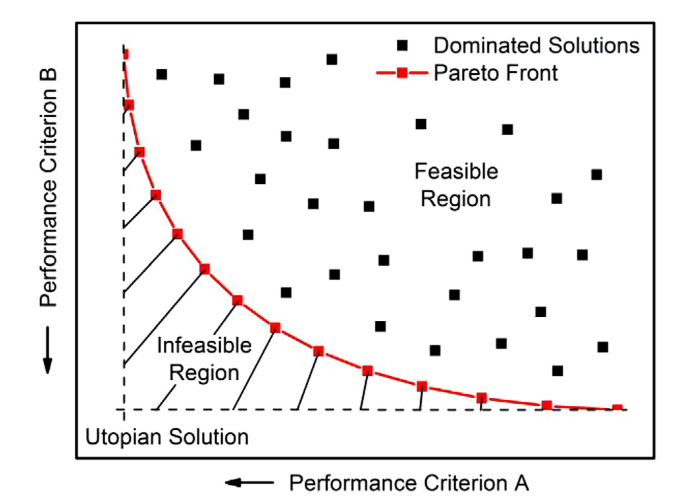
\includegraphics[width=\textwidth]{imatges/domination.png}
    }
    \caption{Explanation of domination [\textit{check memory for citation}] .}
    \label{fig:domination}
\end{figure}

\end{frame}



\begin{frame}{What we need?}
We need an optimization method that:
\begin{itemize}
    \item Can handle mixed-variable problems.
    \item Can handle multi-objective problems.
    \item Can handle non-linear optimization problems.
    \item Can handle find a set of Pareto optimal solutions, i.e. works with a population of solutions.
\end{itemize}
\vspace{1cm}
PROPOSAL: \textbf{NSGA-II: Non-dominated Sorting Genetic Algorithm II}.
\end{frame}


\subsection{NSGA-II Genetic Algorithm}

\begin{frame}{NSGA-II Genetic Algorithm}
\begin{figure}[H]
    \begin{minipage}{0.45\textwidth}
        \centering
        \scalebox{0.35}{
        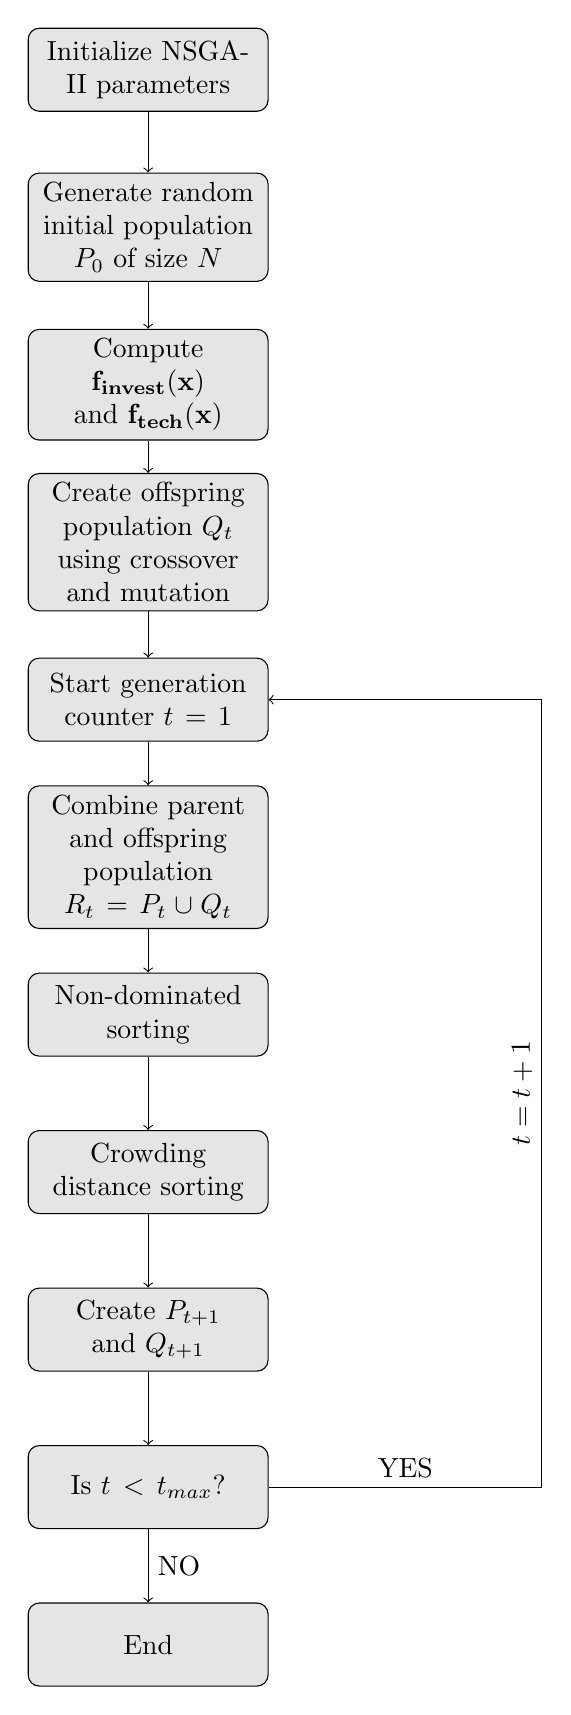
\begin{tikzpicture}[node distance=2cm, auto]
            % Define the style for the boxes
            \tikzstyle{block} = [rectangle, draw, fill=gray!20, 
                                text centered, rounded corners, minimum height=3em, text width= 8em]
        
            \tikzstyle{block3a} = [rectangle, draw, fill=gray!20, 
                                text centered, rounded corners, minimum height=3em, text width=6cm]
        
            % Define the style for the ellipses
            \tikzstyle{block?} = [rectangle, draw, fill=gray!80, 
                                text centered, rounded corners, minimum height=3em, text width=6cm]
        
        
            % Define the nodes
            \node [block] (box1) {Initialize NSGA-II parameters};
            \node [block, below of=box1] (box2) {Generate random initial population $P_0$ of size $N$};
            \node [block, below of=box2] (box3) {Compute $\mathbf{f_{invest}(x)}$ and $\mathbf{f_{tech}(x)}$};
            \node [block, below of=box3] (box4) {Create offspring population $Q_t$ using crossover and mutation};
            \node [block, below of=box4] (box5) {Start generation counter $t=1$};
            \node [block, below of=box5] (box6) {Combine parent and offspring population $R_t = P_t \cup Q_t$};
            \node [block, below of=box6] (box7) {Non-dominated sorting};
            \node [block, below of=box7] (box71) {Crowding distance sorting};
            \node [block, below of=box71] (box72) {Create $P_{t+1}$ and $Q_{t+1}$};
            \node [block, below of=box72] (box8) {Is $t<t_{max}$?};
            \node [block, below of=box8] (box9) {End};
            % Connect the nodes
            \draw [->] (box1) -- (box2);
            \draw [->] (box2) -- (box3);
            \draw [->] (box3) -- (box4);
            \draw [->] (box4) -- (box5);
            \draw [->] (box5) -- (box6);
            \draw [->] (box6) -- (box7);
            \draw [->] (box7) -- (box71);
            \draw [->] (box71) -- (box72);
            \draw [->] (box72) -- (box8);

            \draw [->] (box8) -- node[midway, right] {NO} (box9);
            
            %\draw [->] (box7) to[bend right=80] node[midway,below,sloped] {Optimization method} (box2);
            \draw [->] (box8) -- ++(5,0) node[midway, above] {YES}|-  node[pos=0.25,sloped] {$t=t+1$} (box5);
            
        \end{tikzpicture}
        }
        \caption{NSGA-II algorithm.}
    \end{minipage}
    \begin{minipage}{0.45\textwidth}
        \centering
        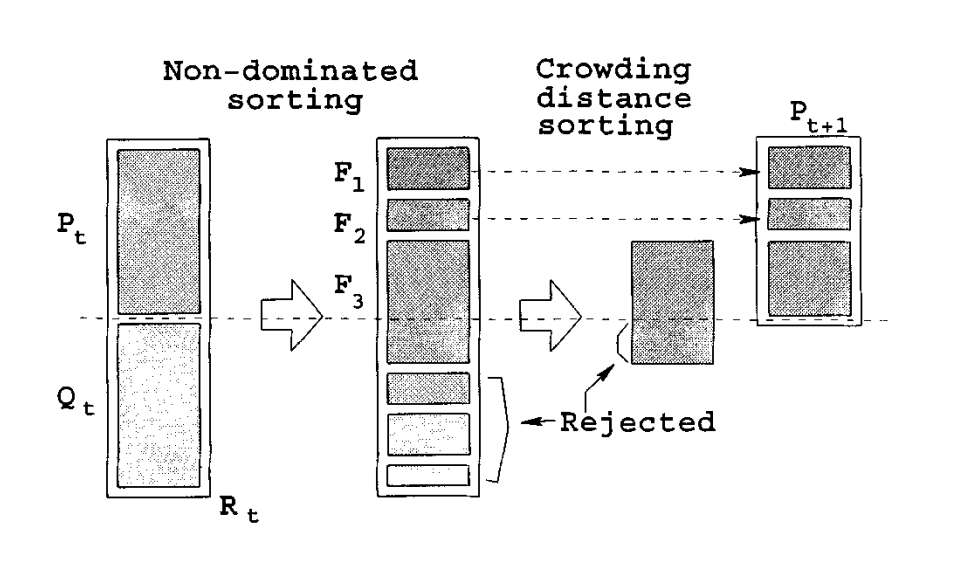
\includegraphics[width=\textwidth]{imatges/proces_nsga.png}
        \caption{Sorting and Crowding process [\textit{check memory for citation}].}
        
      \end{minipage}\hfill
    
\end{figure}

\end{frame}

\begin{frame}{Algorithm overview}

    \begin{figure}[h]
        \centering
        \scalebox{0.40}{
        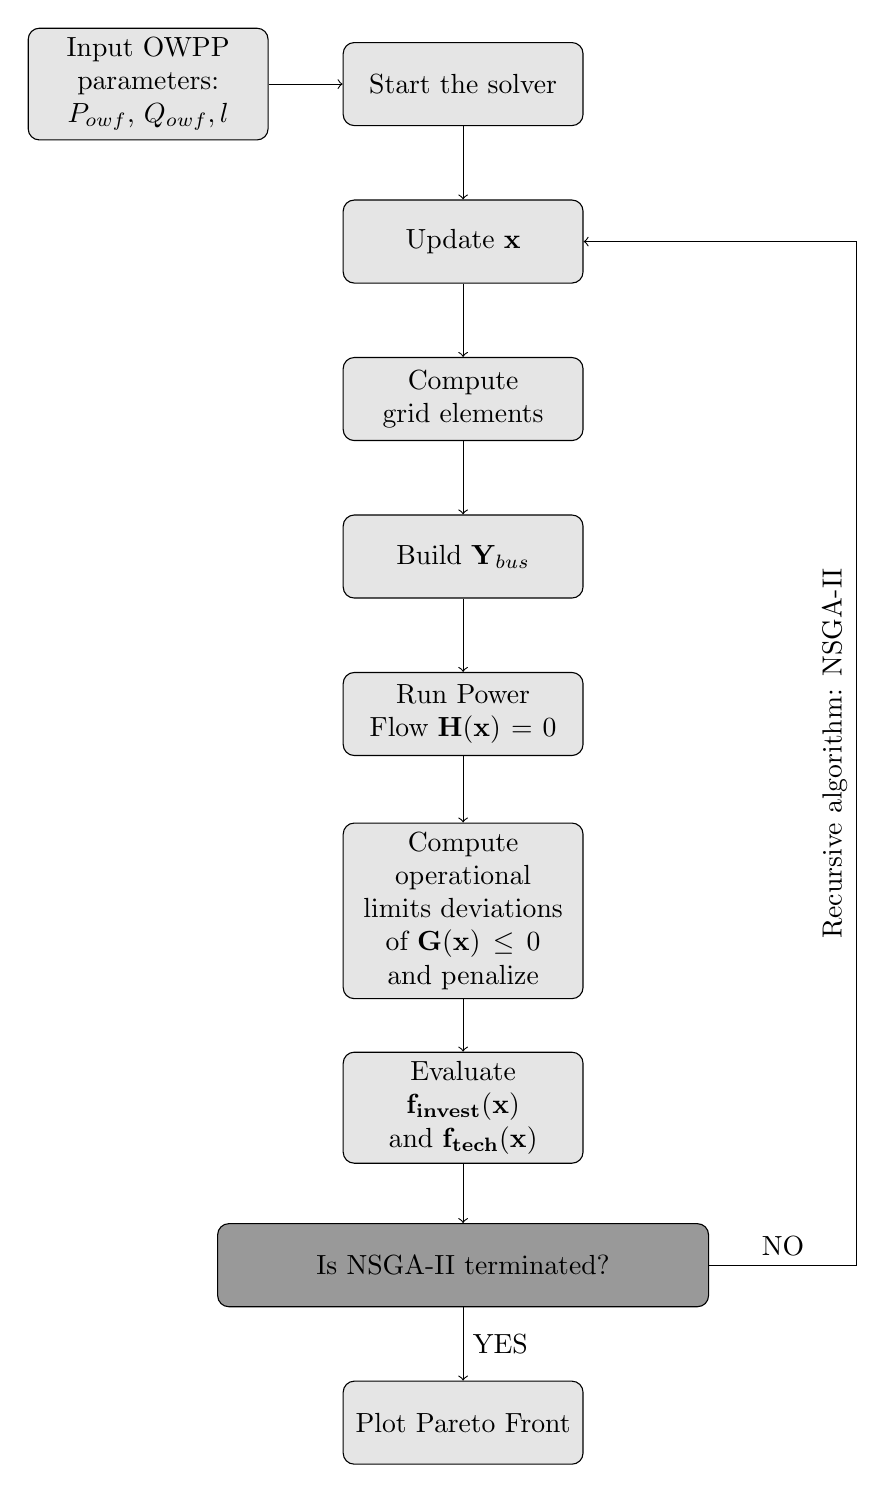
\begin{tikzpicture}[node distance=2cm, auto]
            % Define the style for the boxes
            \tikzstyle{block} = [rectangle, draw, fill=gray!20, 
                                text centered, rounded corners, minimum height=3em, text width= 8em]
        
            \tikzstyle{block3a} = [rectangle, draw, fill=gray!20, 
                                text centered, rounded corners, minimum height=3em, text width=6cm]
        
            % Define the style for the ellipses
            \tikzstyle{block?} = [rectangle, draw, fill=gray!80, 
                                text centered, rounded corners, minimum height=3em, text width=6cm]
        
        
            % Define the nodes
            \node [block] (box1) {Start the solver};
            \node [block, below of=box1] (box2) {Update $\mathbf{x}$};
            \node [block, below of=box2] (box3) {Compute grid elements};
            \node [block, below of=box3] (box4) {Build $\mathbf{Y}_{bus}$};
            \node [block, below of=box4] (box5) {Run Power Flow $\mathbf{H(x)}=0$};
            \node [block, below of=box5, yshift=-0.5cm] (box6) {Compute operational limits deviations of $\mathbf{G(x)} \leq 0$ and penalize};
            \node [block, below of=box6, yshift=-0.5cm] (box7) {Evaluate $\mathbf{f_{invest}(x)}$ and $\mathbf{f_{tech}(x)}$};
            \node [block, left of=box1, xshift=-2cm] (box3a) {Input OWPP parameters: $P_{owf}$, $Q_{owf}, l$};
            \node [block?, below of=box7] (box8) {Is NSGA-II terminated?};
            \node [block, below of=box8] (box9) {Plot Pareto Front};
            % Connect the nodes
            \draw [->] (box1) -- (box2);
            \draw [->] (box2) -- (box3);
            \draw [->] (box3) -- (box4);
            \draw [->] (box4) -- (box5);
            \draw [->] (box5) -- (box6);
            \draw [->] (box6) -- (box7);
            \draw [->] (box3a) -- (box1); % New arrow
            \draw [->] (box7) -- (box8);
            \draw [->] (box8) -- node[midway, right] {YES} (box9);
            
            %\draw [->] (box7) to[bend right=80] node[midway,below,sloped] {Optimization method} (box2);
            \draw [->] (box8) -- ++(5,0) node[midway, above] {NO}|-  node[pos=0.25,sloped] {Recursive algorithm: NSGA-II} (box2);
            
        \end{tikzpicture}
        }
        \caption{Proposed optimization algorithm.}
        \label{fig:block_overview}
        \end{figure}
    
\end{frame}


\subsection{OPF Validation}
\begin{frame}{OPF for reactor sizing validation}

We modify the traditional AC-OPF objective function of minimizing cost of generating active power, $P_G$, for minimizing $C_{sh}$, reactive power compensation cost, while satisfying the constraints:
\begin{equation}\label{eq:Qopf}
    \underset{Q_{sh}}{\text{min}} \quad \mathbf{c_{sh}^T} \mathbf{Q_{sh}} \quad \text{where} \quad \mathbf{c_{sh}} = \begin{bmatrix} K \\ P \\ 0 \end{bmatrix}
    \end{equation}

where $K$ and $P$ come from the cost function of the shunt reactors:
\begin{equation}\label{eq:shuntcost}
    C_{sh}= K \cdot Q_{sh} + P = K \cdot Y_{sh}\cdot U_{AC-N}^2 + P \quad  \text{[M€]} 
\end{equation}

\begin{table}[H]
    \centering
    \begin{tabular}{c|c|c}
    \hline
    \textbf{Location} & \textbf{K} & \textbf{P} \\
    \hline
    Onshore & 0.01049 & 0.8312  \\
    Offshore & 0.01576 & 1.244 \\
    Mid-cable & 0.01576 & 12.44 \\
    \hline
    \end{tabular}
    \caption{K and P for different positions of the shunt reactors [\textit{check memory for citation}].}
    \label{tab:parametersshunt}
    \end{table}
\end{frame}






\section{Results}

\begin{frame}{}
    \tableofcontents[currentsection]
\end{frame}




\section{Conclusions}
\begin{frame}{}
    \tableofcontents[currentsection]
\end{frame}

% \begin{frame}{Conclusions}
%     \begin{itemize}
%         \item A new classification of buses has been proposed. A modified Newton-Raphson algorithm that considers the current equation of converters has been developed.
%         \item It has been found possible in a simple system to algebraically include the current limits of converters with a formulation based on a Lagrangian.
%         \item The voltage-support provided by conventional grid codes can be improved. The adapted grid codes are concluded to be near-optimal.
%         \item The Galerkin method has been studied. A generalized program to solve realistic grids with small errors has been written. 
%         \item The Principal Component Analysis (PCA) combined with dimension reduction yields satisfactory errors and is much more efficient than the Galerkin method. The parametrized states can be used in optimization problems.
%     \end{itemize}
% \end{frame}

\begin{frame}{Conclusions}
    \textcolor{green}{\ding{51}} To analyze voltage spread of distribution grid with high penetration of solar.

    \textcolor{green}{\ding{51}} To develop a dynamic model of the UPQC, including all required controllers.

    \textcolor{green}{\ding{51}} To develop an equivalent static model of the UPQC and validate its behaviour with the dynamic model.

    \textcolor{green}{\ding{51}} To propose design methodology for the converter sizing making use of the developed tools.

    \textcolor{green}{\ding{51}} To show behaviour of the converter over sample days using different design criteria.
\end{frame}



\begin{frame}{Next Steps}
    \begin{itemize}
        \item Find optimal shunt converter current calculation
        \item Extend static model to state space to provide pseudo dynamic behaviour
        \item Create a voltage limit condition dependent on the load
    \end{itemize}
\end{frame}

% \begin{frame}{Future work}
%     \begin{itemize}
%         \item To develop heuristics to determine the states of the converters and how to switch between them in order to get to a solution.
%         \item To develop the Lagrangian formulation for AC systems in order to realistically include converters' current limits.
%         \item Study the optimality of grid codes in distribution grids.
%         \item Parametrize the fault impedances instead of the powers. This way, obtaining results for a sweep of fault impedances could be significantly faster.
%         \item Test other families of bases for the Galerkin method such as Chebyshev polynomials.
%     \end{itemize}
% \end{frame}






\begin{frame}[plain]
\hspace*{-1.0cm}\parbox[t]{\textwidth}{
	\titlepage
    } 
\end{frame}


\end{document}

